\chapter[Measurements]{Measurements}


The measurements can, to a certain extent, be broken into three main components: those pertaining to the solar wind and solar corona, those from the magnetosphere in general, and those specific to the plasmasphere. The combined data sources used in this dissertation are shown in Figure \ref{fig:alldata-GOES6-1983-1991}, providing solar wind variables $B_z$ and $V_{SW}$, solar variable $F_{10.7}$, plasmatrough variable \req, and magnetosphere variable \dst.

\begin{figure}[htp!]
	\centering
	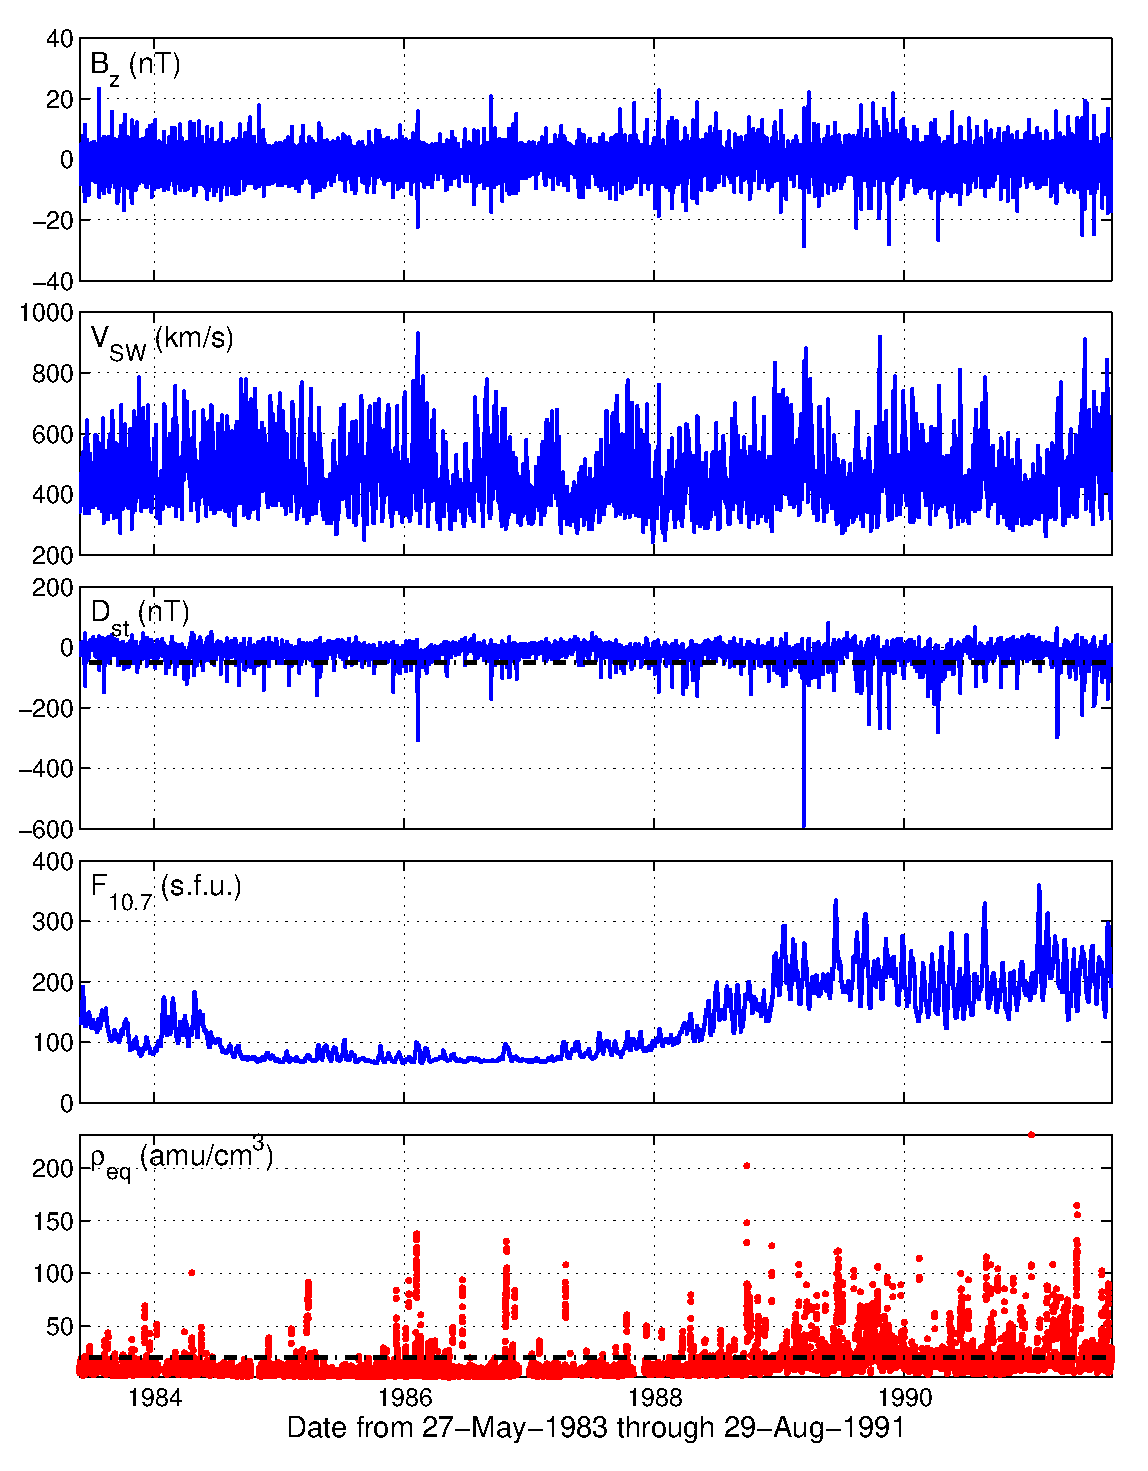
\includegraphics[width=1\linewidth]{Figures/alldata-GOES6-1983-1991}
	\caption{Data from GOES 6 with dashed lines indicating default event thresholds discussed in Chapter 4.}
	\label{fig:alldata-GOES6-1983-1991}
\end{figure}

Similarly, Figure \ref{fig:alldata-GOES6-1989-1989} earlier showed the same variables before, during, and after the March 1989 geomagnetic storm as seen by GOES 6. This makes it clearer how the variables are interrelated, notably how short-timescale effects such as drops in $B_z$ and \dst\ are connected, or longer time scale changes in $F_{10.7}$ and $V_{SW}$ are related. It also shows how the sparse availability of \req\ created challenges for this study, which is discussed in more detail later in Section \ref{DataSparsity} . 

Figure \ref{fig:alldata-examples} shows four more selected examples of short time periods with interesting characteristics. They all show, to a varying degree, an elevated solar wind velocity coinciding with a drop in \dst, and almost always also an enhancement in southward $B_z$. The bottom right panel also appears to show how an extended period of no activity allows the plasmasphere to refill.


\begin{figure}[htp!]
	\centering
	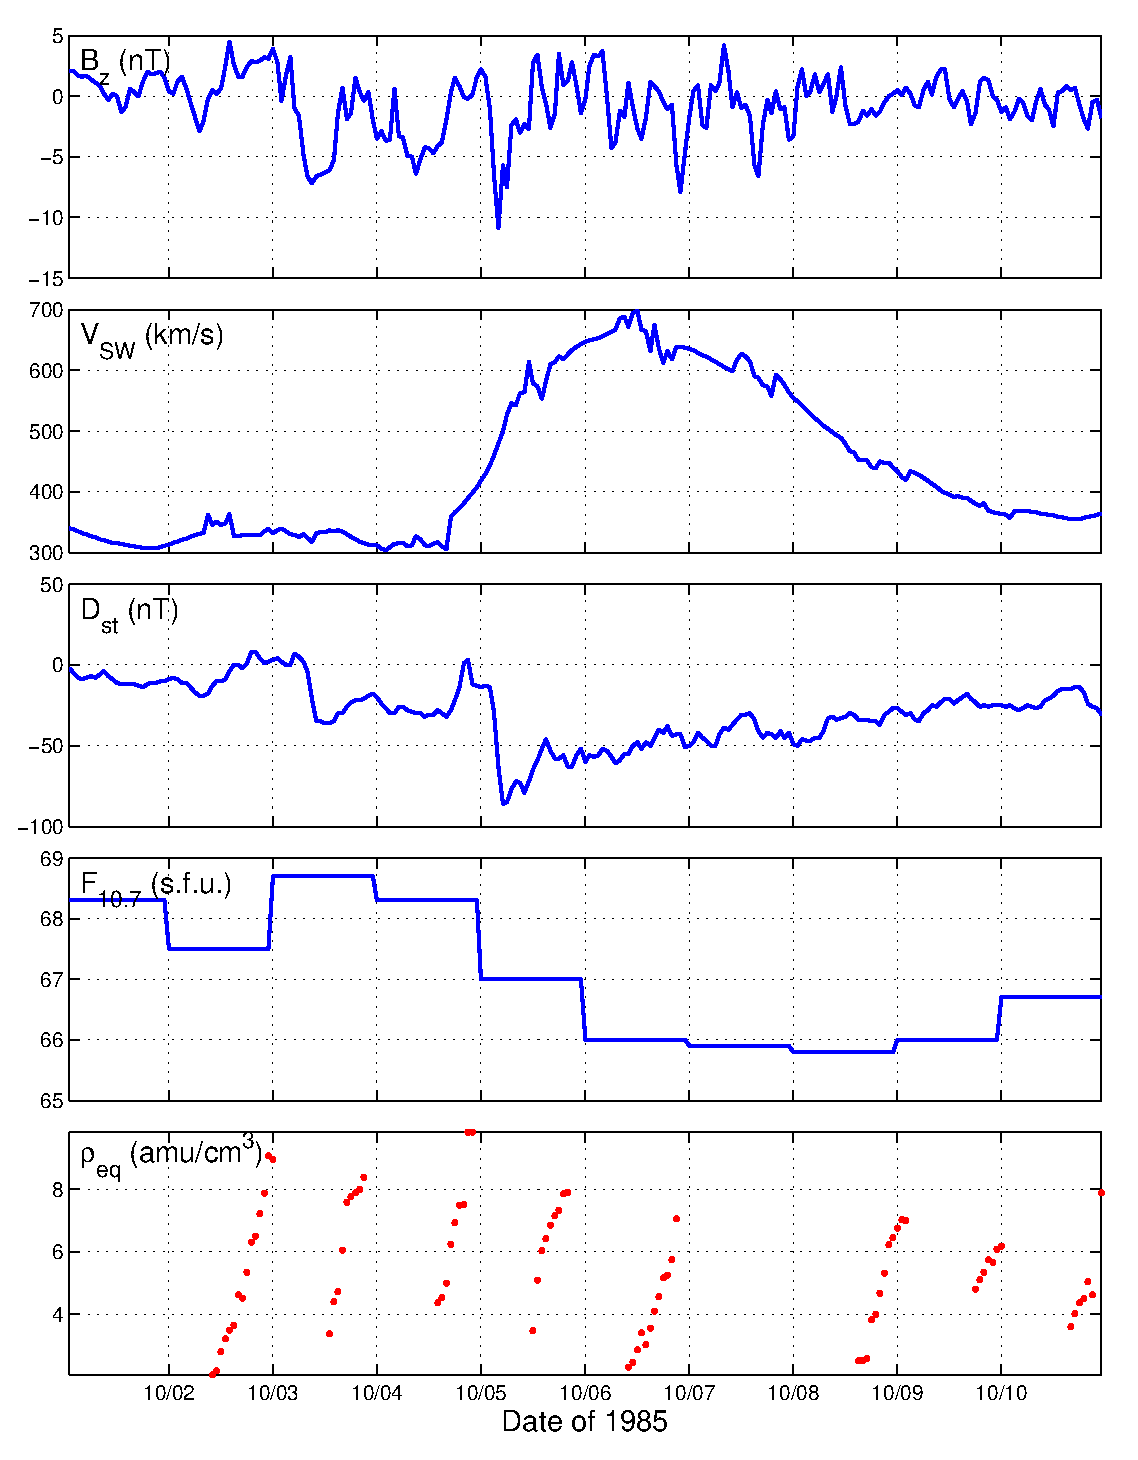
\includegraphics[width=0.45\linewidth]{Figures/alldata-GOES6-01Oct1985-10Oct1985}
	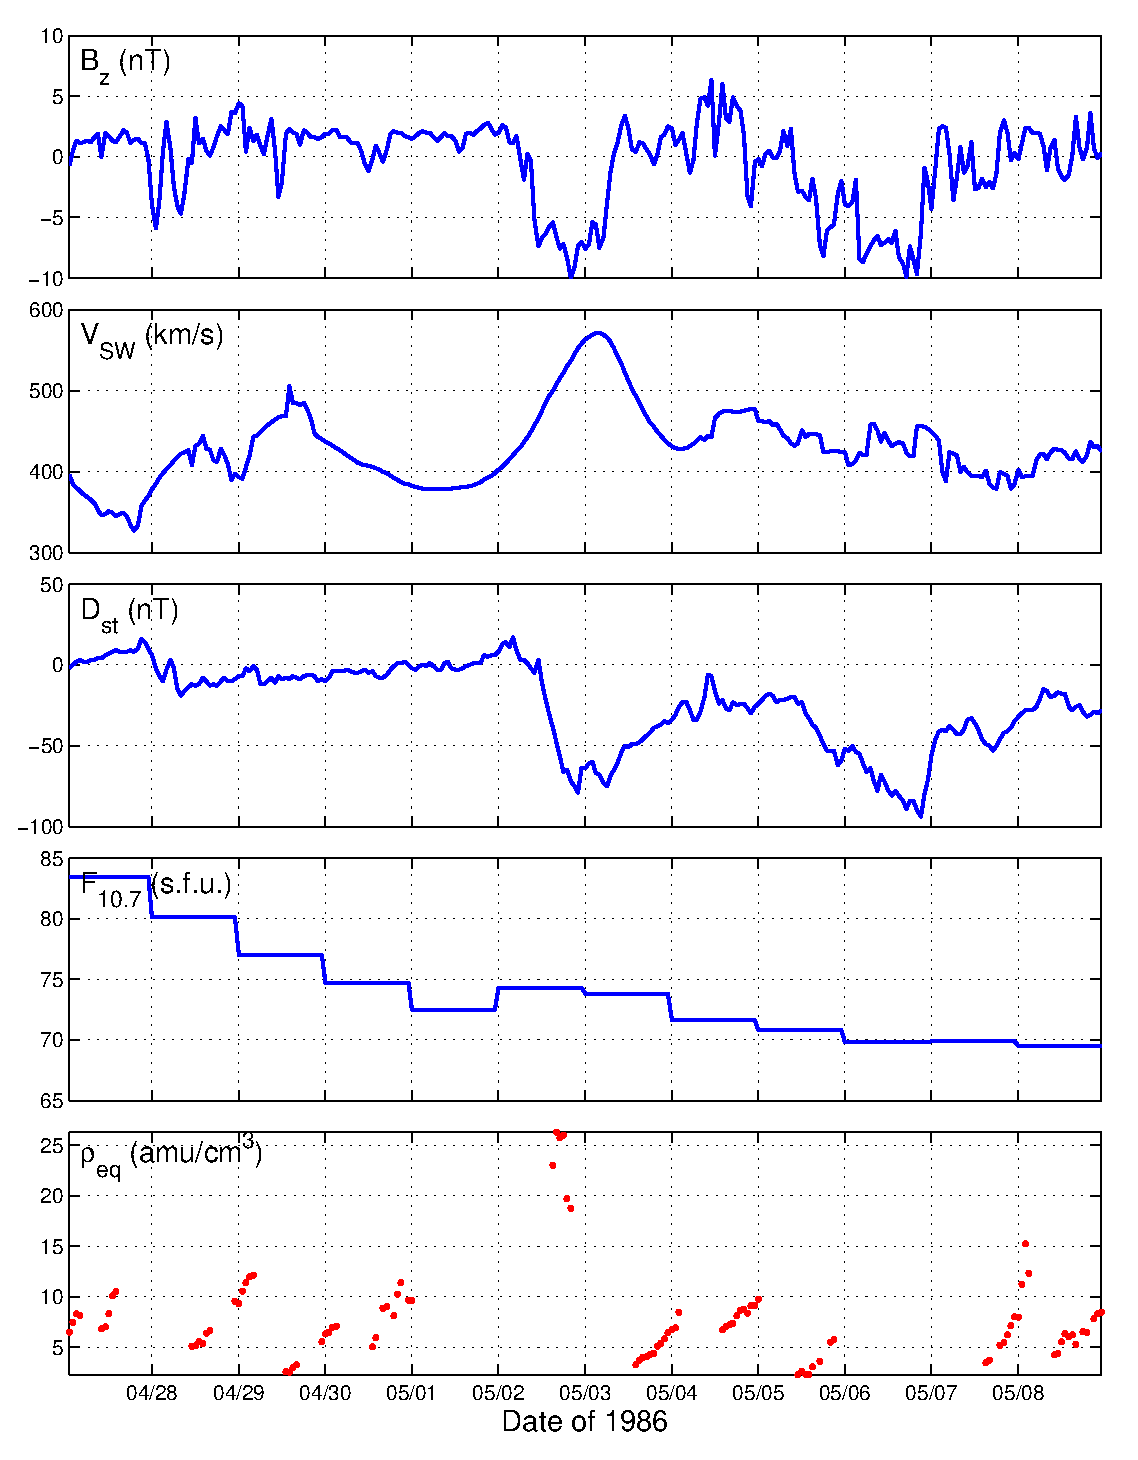
\includegraphics[width=0.45\linewidth]{Figures/alldata-GOES6-27Apr1986-08May1986}
	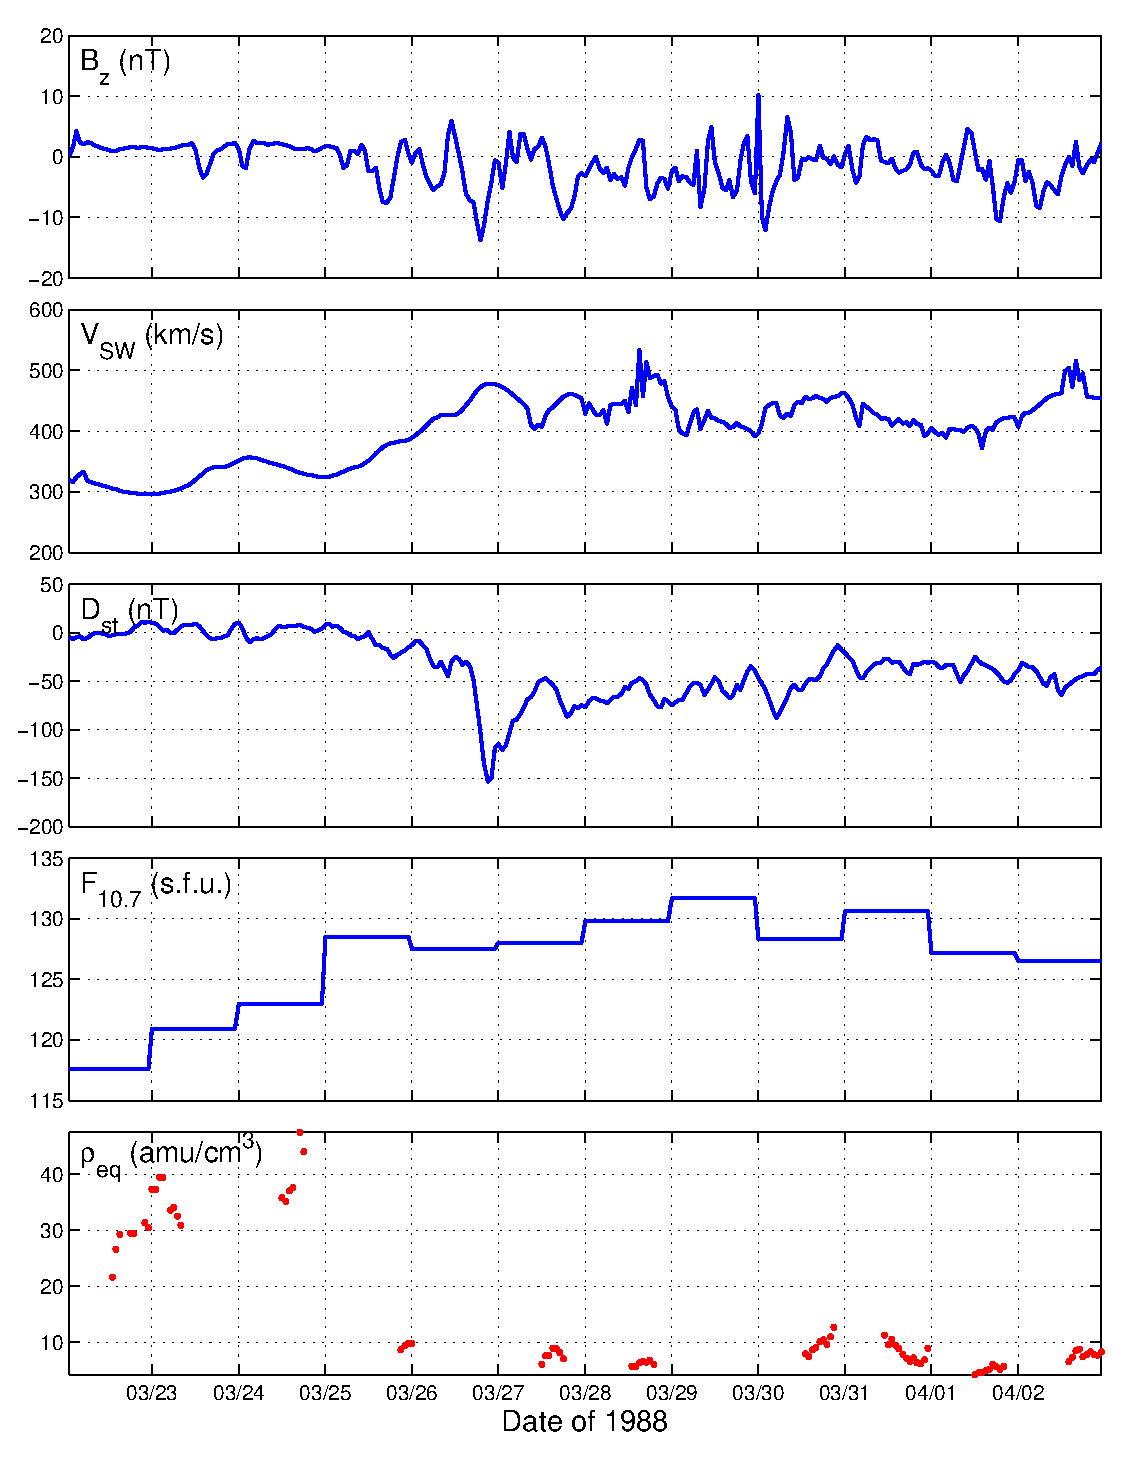
\includegraphics[width=0.45\linewidth]{Figures/alldata-GOES6-22Mar1988-02Apr1988}
	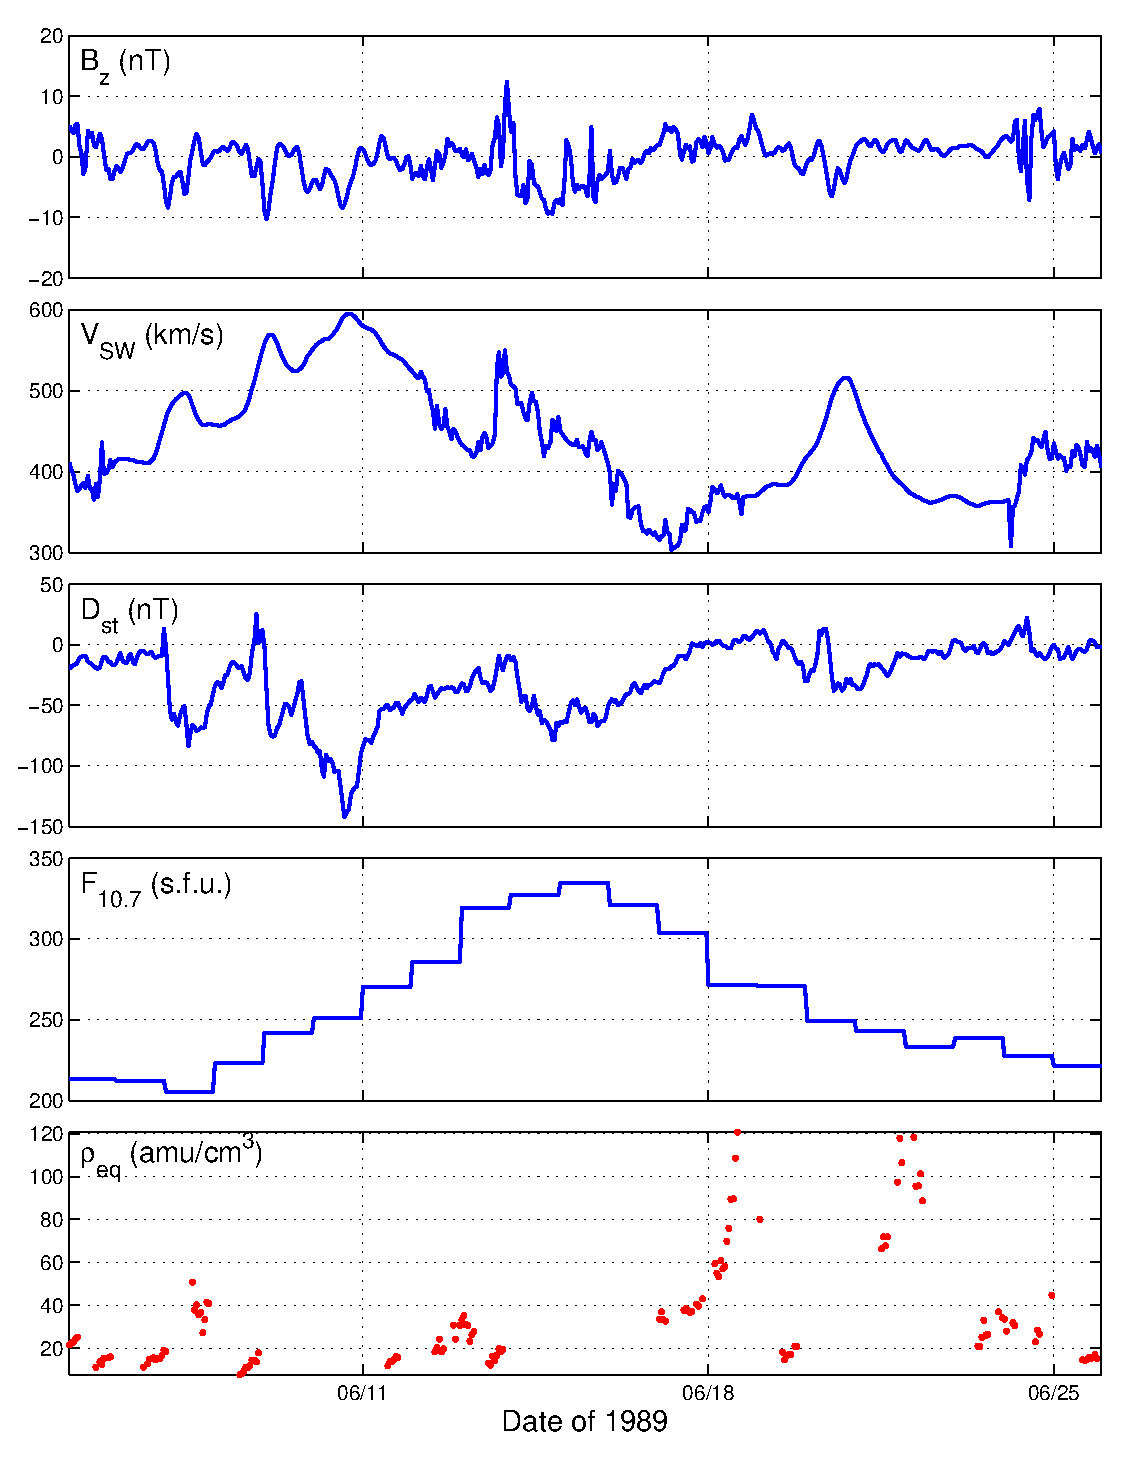
\includegraphics[width=0.45\linewidth]{Figures/alldata-GOES6-05Jun1989-25Jun1989}
	\caption{Four examples of specific events from GOES 6.}
	\label{fig:alldata-examples}
\end{figure}




%K>> starti(~isnan(AVMDMat(:,28)))
%20689       24335       25706       42384
%K>> datestr(FILLEDTime(20689))
%05-Oct-1985 16:00:00  %Reall good CIR?
%K>> datestr(FILLEDTime(25706))
%02-May-1986 17:00:00
%K>> datestr(FILLEDTime(42384))
%27-Mar-1988 15:00:00

\section{Solar Wind}
The solar wind is the primary source of particles for the magnetosphere, and as such is an important input for a plasmatrough model. Conditions such as magnetic field orientation and particle velocity are important considerations for whether the plasmasphere is expected to be compressed, saturated, or experiencing high variability. By adding these to a model that includes time delayed inputs, their effects can be accounted for and aid in categorizing the state of the plasmatrough.

\subsection{Source}
Solar wind data for this dissertation is provided by the OMNIWeb service \citep{OMNIWebKing2005}, which contains data from multiple satellites and is uniform in time, supplying a near-Earth set of solar wind measurements. The one-hour resolution dataset was used since the study is concerned with effects on timescales of longer than an hour, and to more easily compare to the other data sources used. 

Since the OMNIWeb data has gaps for some of the variables, the dataset developed for \cite{Kondrashov2014ReconstructionOfGaps} was used as they reliably reconstruct gaps to make a continuous, uniform data set. They used Singular Spectrum Analysis to create a set of principle components and empirical orthogonal functions to find that the data contained significant oscillatory modes. This allowed the reconstruction of gaps in solar wind driving variables by using continuously observed responses such as geomagnetic indices.

\subsection{Coverage}
Low resolution (1-hour cadence) OMNI data is available from 1963 to present, but only the years of 1983-1992 were considered as they overlapped with the other data sets of interest. The data covers, but is not limited to: magnetic field magnitude in all three dimensions; solar wind proton density and temperature; and the $K_p$, $AE$, $F_{10.7}$, and $D_{st}$ indices.

\subsection{Data preparation}
The only data cleaning required on the OMNI dataset was to convert fill values of 999.9 and 9999 to NaN, to be appropriate for use in data analysis so they would not be included in calculations. Of the variables included (see Coverage), $B$, $B_z$ (GSE and GSM), and Solar wind proton number density and plasma speed all were missing about 35\% of their data. The $AE$ index was missing about 7\% of its data, and all other variables had no time gaps.

\section{Geomagnetic}
Geomagnetic data cover everything inside the magnetopause, extending out to a distance of roughly 10$R_E$ on the sunward side of Earth. 

\subsection{Source}
The data come from \cite{Takahashi2010SolarCycleVariation}, which takes data from the Geostationary Operational Environmental Satellites (GOES) and uses a set of magnetic field models to relate Alfvén waves to equatorial mass density (\req). By taking magnetic field vectors and applying spectral analysis, they find a set of fundamental harmonic frequencies of toroidal waves. Through testing, they find a strong linear dependence of the 27-day average third toroidal frequency ($f_{T3\_27d}$) on the similarly averaged $F_{10.7}$ index, of the form: $f_{T3\_27d}(mHz)=37.5-0.0972 F_{10.7\_27d}(sfu)$. From there, they also find a linear relationship to the averaged \req\ in the form $\log_{10}(\rho_{eq\_27d})=0.421+0.00390 F_{10.7\_27d}$, effectively linking the derived toroidal frequency to \req.

\subsection{Coverage}
\label{DataSparsity}
The GOES satellites used in this study cover the years from 1980 to the end of 1991, often with overlapping years between satellites. The satellites themselves held a geostationary orbit at around 6.62 $R_E$ and collected data on a roughly 3-second cadence \citep{GOESDataSource}, which was then transformed onto a 10-minute cadence. Their radial position means they are almost always measuring properties of the plasmatrough, the region devoid of dense plasma located just outside the plasmasphere. Figure \ref{fig:PlasmapauseLocation} shows the location of the GOES satellites relative to the magnetopause in the top panel, while also showing that the plasmapause location tends to vary from 2-6 $R_E$ depending on magnetic activity.

\begin{figure}[htp!]
	\centering
	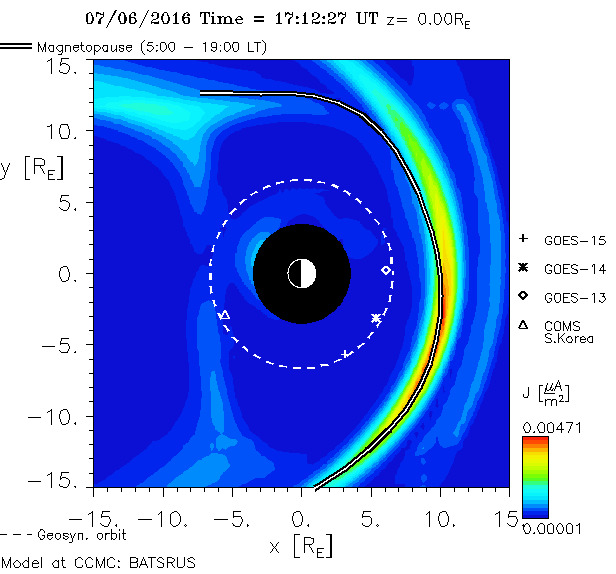
\includegraphics[width=0.9\linewidth]{Figures/iSWACygnetStreamer.jpg}
	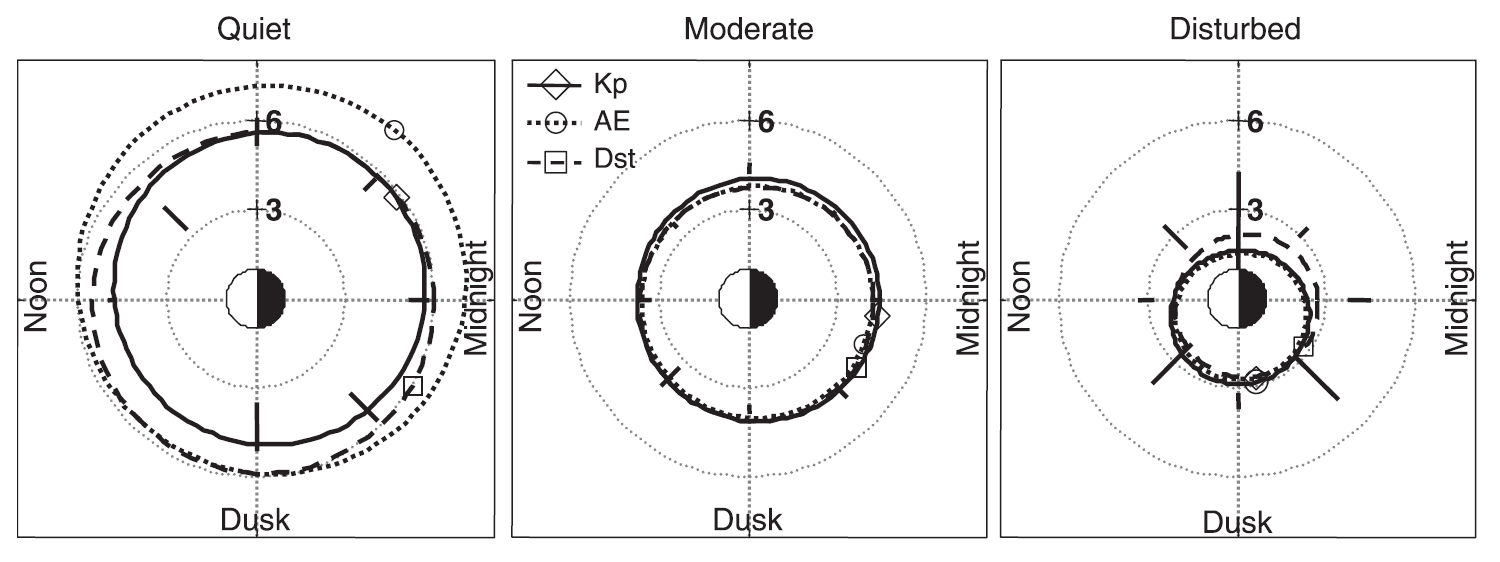
\includegraphics[width=0.9\linewidth]{Figures/PlasmapauseLocation.png}
	\caption{Top: Model of magnetopause location showing location of GOES satellites in geosynchronous orbit \citep{CCMC}, taken during a period of $K_p$=4. Bottom: Model of plasmapause location as it varies with geomagnetic activity where the symbols indicate the local time of maximum plasmapause location \citep{OBrien2003EmpiricalPlasmapause}.}
	\label{fig:PlasmapauseLocation}
\end{figure}

\subsection{Data preparation}
The data were prepared by replacing fill values of 9999 with NaN and then narrowing results to only one satellite at a time to ideally remove any effects of satellite position or calibration from the results. These data still had many temporal gaps (roughly 22\% of the 10-minute intervals between the first and last point of GOES 6 had any data, since the detection rate of the relevant frequency in the toroidal waves ($f_{T3\_30m}$) varied with local time, magnetic latitude, and the strength of the compressional source waves \citep{Takahashi2010SolarCycleVariation}), so they were placed onto a uniform 10-minute grid leaving missing points as NaN, allowing for easier data analysis and comparison to other data sets. The detection rate as a function of magnetic latitude and magnetic local time is shown in Figure \ref{fig:Takahashi2010Availability}.

\begin{figure}[htp!]
	\centering
	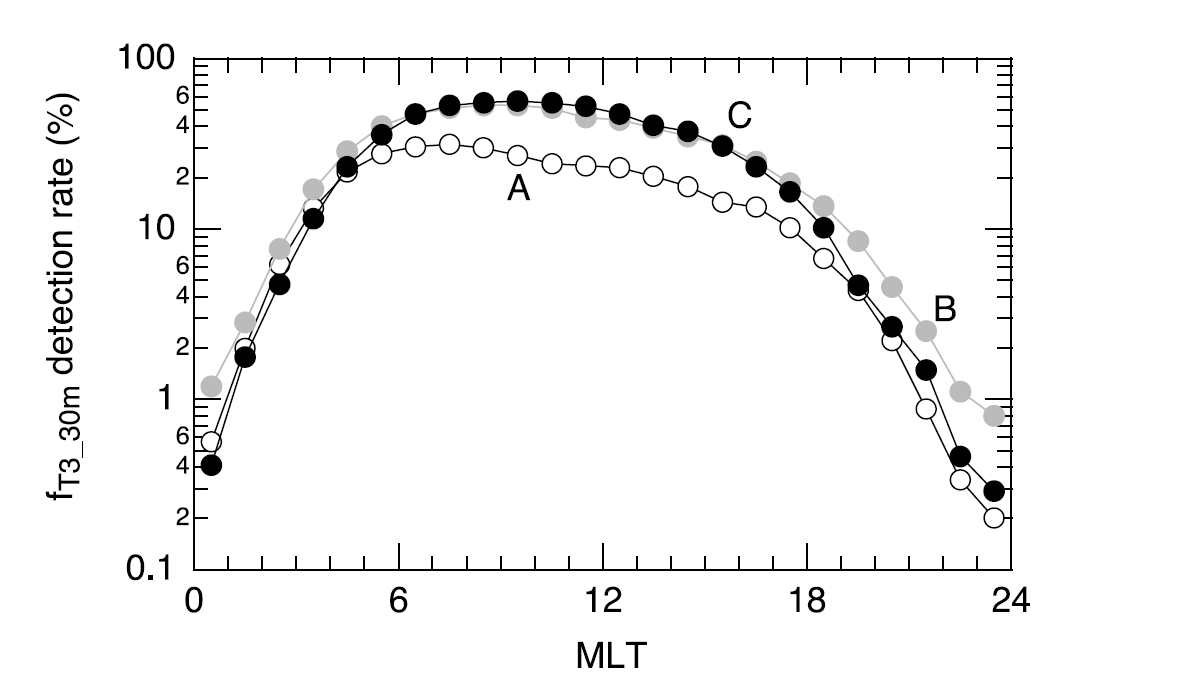
\includegraphics[width=0.8\linewidth]{Figures/Takahashi2010Availability.png}
	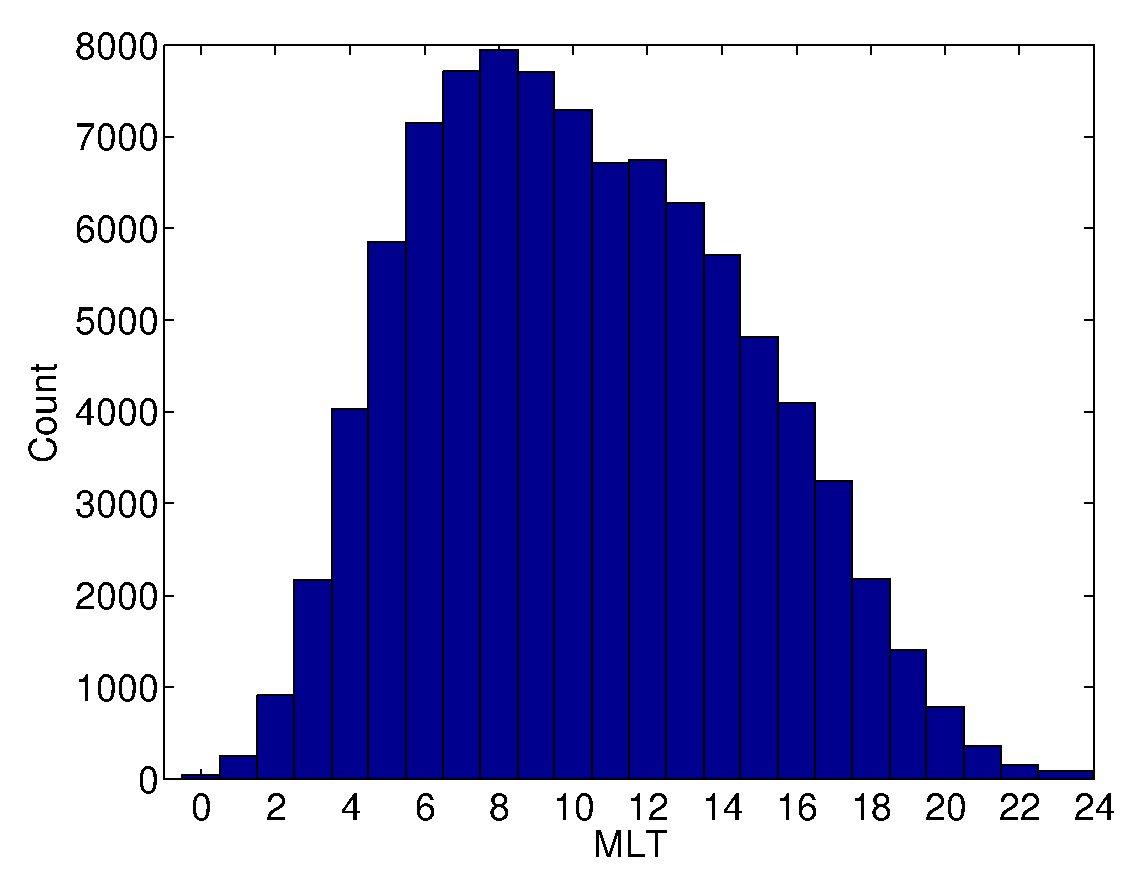
\includegraphics[width=0.8\linewidth]{Figures/databyMLT}
	\caption{Top: Detection rate of $f_{T3\_30m}$ for magnetic latitudes of 5, 9, and 11 degrees (curves A, B, and C respectively) \citep{Takahashi2010SolarCycleVariation}. Bottom: MLT of all available data.}
	\label{fig:Takahashi2010Availability}
\end{figure}


In order to align the GOES data with the OMNI 1-hour cadence, the median of all existing 10-minute values within an hour was treated as the value for that hour (i.e. the median of all values from 7:00-7:59 was the value for 7:00). This was done to match the OMNI standard, and showed no significant difference on our timescales as using a centered median. For hours with no existing values, a NaN was inserted to keep the cadence uniform. 

\section{Plasmasphere and Plasmatrough}
Plasmasphere data covers the inner regions of the magnetosphere, bounded by the plasmapause on the outer edge and the ionosphere on the inner edge. This puts it at a typical distance of $L=3-5R_E$ \citep{Carpenter1992ISEEModel}. 

\subsection{Source}
Data for the plasmasphere also comes from the GOES and OMNI datasets previously discussed, but are often calculated as extensions of directly measured data either onboard the satellites or from ground stations, depending on the current extent of the plasmasphere and location of the satellite.

\subsection{Coverage}
Since the data come from the same sources as that of the magnetosphere, the coverage is largely the same with specifics covered in \cite{Takahashi2010SolarCycleVariation}, as the satellites used most often reside in the plasmatrough. Figure \ref{fig:PlasmatroughLocation} shows the typical locations of the plasmapause, and how this puts the GOES satellites firmly in the plasmatrough at 6.6$R_E$.

\begin{figure}[htp!]
	\centering
	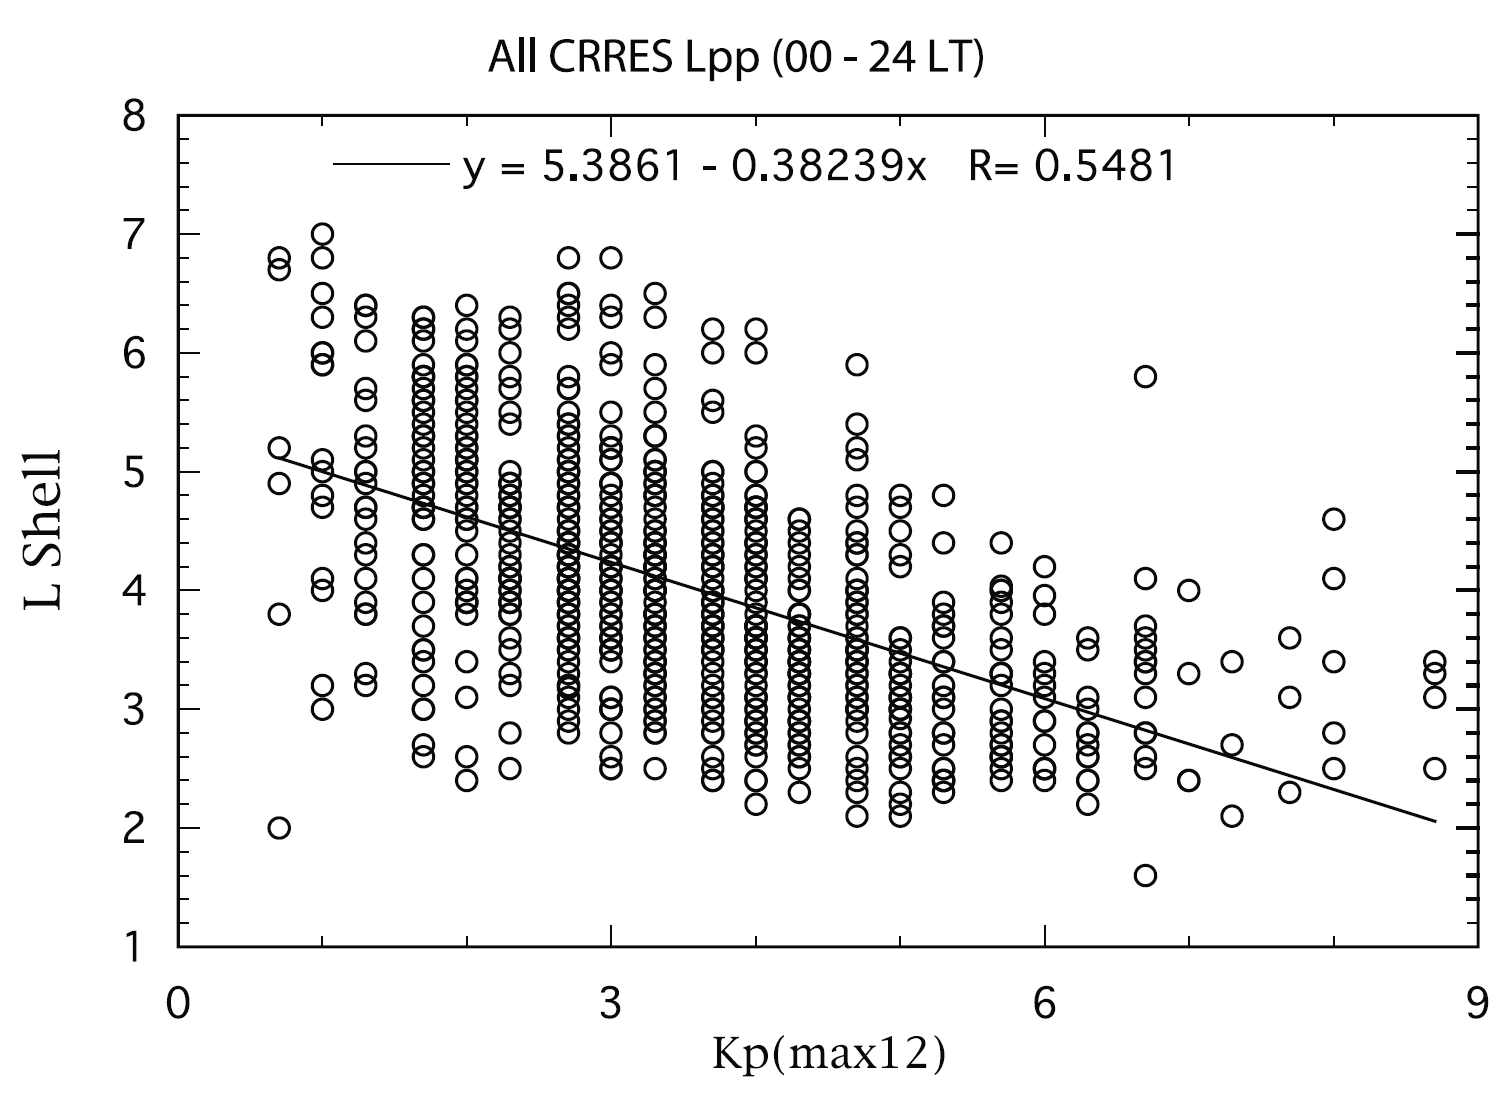
\includegraphics[width=0.8\linewidth]{Figures/LShellPlasmapuse.png}
	\caption{Location of detected plasmapause on CRRES against the maximum $K_p$ value for the previous 12 hours \citep{Moldwin2002ModelPlasmapause}.}
	\label{fig:PlasmatroughLocation}
\end{figure}



\subsection{Data preparation}
The same preparation done for the magnetosphere applied to the plasmasphere data.  Some specific analysis done in \cite{Takahashi2010SolarCycleVariation} discusses how the spacecraft's geomagnetic location affected their ability to detect the necessary toroidal frequency, and thus estimate \req, so for some of the long-timescale averages, only certain MLTs were included. They also show that \req\ inversely correlates with geomagnetic activity (and, by extension, plasmapause location), so during long periods of no activity the plasmasphere extends beyond geosynchronous orbit, leading to measurements of \req\ reflecting density in the plasmasphere and not the plasmatrough. 

